\documentclass{article}
\usepackage[utf8]{inputenc}
\usepackage[spanish]{babel}
\usepackage{amsfonts}
\usepackage{design_ASC}
\usepackage{caption}

\usepackage{amsmath}
\usepackage{graphicx}
\usepackage[colorinlistoftodos]{todonotes}

\usepackage{underscore}

\begin{document}
\begin{titlepage}
    \begin{center}
        \vspace*{1cm}

        
\includegraphics[width=0.22\textwidth]{img/universidadDelValle.png}
        
        \vfill
        \textbf{Proyecto final - PPR}\\
        \vfill
        
        Estudiantes\\
        Jhon Henry Carabalí Miranda cod. 201910001\\
        Jose Manuel Madrid Torres cod. 201943827\\
        Sebastián Afanador Fontal cod. 1629587\\
        \vfill
        Profesor\\
        Profesor Juan Francisco Diaz Ph.D.\\
        
        \vfill

        \textbf{Programación por restricciones}
        
        \vfill
           
        Escuela de Ingeniería de Sistemas y Computación -EISC\\
        Facultad de Ingeniería\\
        Universidad del Valle\\
        Cali - Colombia\\
        \vfill
        \date{05 de Agosto del 2022}

    \end{center}
\end{titlepage}
\section{Modelo básico}
Un estudio de grabación desea optimizar el tiempo que contrata a un grupo de actores $A$ para grabar una telenovela titulada "Desenfreno de Pasiones", esta telenovela tiene un conjunto de escenas $E$ que deben ordenarse para cumplir con el requerimiento mencionado de manera que sea mínimo el tiempo que cada actor debe estar en el estudio. Dicho de otra manera el orden importa porque el tiempo de permanencia . \newline

A continuación se describen los elementos que componen el problema según el paradigma de programación por restricciones.

\subsection{Parámetros de entrada}
\begin{itemize}
    \item $ACTORES$: Es el conjunto de los nombres de los actores de la telenovela.
    \item $n\textunderscore actores \in \mathbb{N}$: Es la cantidad de actores de la telenovela $n(ACTORES)$, es decir, la cardinalidad de $ACTORES$.
    \item $Duracion$: Es el conjunto de las duraciones de las escenas de la telenovela en unidades de tiempo con $Duracion_i \in \mathbb{N}$ donde $i \in [1..n\textunderscore escenas]$.
    \item $n\textunderscore escenas \in \mathbb{N}$: Es la cantidad de escenas de la telenovela $n(Duracion)$, es decir, la cardinalidad de $Duracion$.
    \item $Escenas$: Es la participación que tienen los actores en las escenas con $escena_{i,j} \in \{0,1\}$ cuando $j < n\textunderscore escenas + 1 $ donde  $1$ representa que el actor participa en la escena y $0$ no participa. $escena_{i,j}$ representa la participación del $i-esimo$ actor con $i \in [1..n\textunderscore actores]$ para la $j-esima$ escena con $j \in [1..n\textunderscore escenas + 1]$ donde el valor $escena_{i,n\textunderscore escenas + 1}$ corresponde al precio que cobra el actor $i$ por unidad de tiempo.
\end{itemize}

\subsection{Variables}
\begin{itemize}
    \item $orden\textunderscore escenas$: Representa el orden que deben tener las escenas de la telenovela para para minimizar el $costo\textunderscore total$. Es el conjunto de las escenas donde $orden\textunderscore escenas_i \in [1..n\textunderscore escenas]$ con $i \in [1..n\textunderscore escenas]$ son cada una de las posiciones en orden cronológico de las escenas.
    \item $Escenas\textunderscore$: De manera similar que $Escenas$, $Escenas\textunderscore$ es la información de la participación de los actores en las escenas donde $escena\textunderscore_{i,j} \in \{0,1\}$ representa la participación del $i-esimo$ actor con $i \in [1..n\textunderscore actores]$ para la $j-esima$ escena con $j \in [1..n\textunderscore escenas + 1]$ donde  $1$ representa que el actor participa en la escena y $0$ no participa. $Escenas\textunderscore$ se ordenará con respecto a $orden\textunderscore escenas$. Esta variable se crea con el fin de mostrar la matriz solución y así dar una mejor representación de la solución de un problema.
    \item $costo\textunderscore x\textunderscore actor$: Son los valores que cobrarán cada uno de los actores con $costo\textunderscore x\textunderscore actor_i \in \mathbb{N}$ donde $ i \in [1..n\textunderscore actores]$ con base al $orden\textunderscore escenas$ que minimice el $costo\textunderscore total$.
    \item $costo\textunderscore total \in \mathbb{N}$: Esta variable representa el costo total mínimo que debería tener la grabación de la telenovela.
\end{itemize}

\subsection{Funciones}
\begin{itemize}
    \item $primera\textunderscore escena(actor)$: Es la primera escena en la que participa un $actor \in [1..n\textunderscore actores]$ con base al nuevo orden de las escenas dado por $Escenas\textunderscore$.
    \item $ultima\textunderscore escena(actor)$: Es la primera escena en la que participa un $actor \in [1..n\textunderscore actores]$ con base al nuevo orden de las escenas dado por $Escenas\textunderscore$.
\end{itemize}

\subsection{Restricciones}
\begin{itemize}
    \item $\forall i \nexists j$ tal que $i = j$ \newline donde $i \land j \in orden\textunderscore escenas$
    \item $\forall i 1 \leq orden\textunderscore escenas_i \leq n\textunderscore escenas$  donde $i \in orden\textunderscore escenas$.
    \item $\forall i \forall j$  $Escenas\textunderscore_{i,j} = Escenas[i,orden\textunderscore escenas_{j}]$ \newline donde $i \in [1..n\textunderscore actores] \land j \in [1..n\textunderscore escenas]$.
    \item $\forall i\sum_{j=primera\textunderscore escena(i)}^{ultima\textunderscore escena(i)}$  $Duracion[orden\textunderscore escenas_j] * Escenas_{i,n\textunderscore escenas+1} = costo\textunderscore x\textunderscore actor$\newline
          donde $i \in [1..n\textunderscore actores]$.
\end{itemize}

\subsection{Función objetivo}
\begin{itemize}
    \item $min(\sum_{i=1}^{n\textunderscore actores}costo\textunderscore x\textunderscore actor$)
\end{itemize}

\subsection{Pruebas}
A continuación se presentan los escenarios de pruebas a los que se sometió el modelo usando Minizinc, el equipo usado para correr las pruebas tiene un procesador Intel(R) Core(TM) i7-10510U CPU @ 1.80GHz   2.30 GHz con 16.0 GB (15.8 GB usable) de RAM DDR4 bus 2400MHz.\newline
Se adjuntan los escenarios de prueba.

\subsubsection{test01_m1_a3_e5.dzn}
\begin{center}
    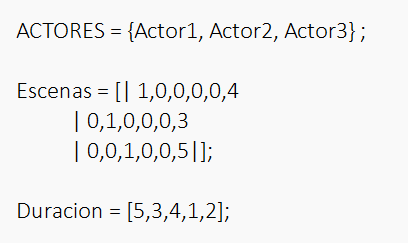
\includegraphics[width=0.35\textwidth]{img/test01_m1.png}
\end{center}

\subsubsection{test02_m1_a4_e5.dzn}
\begin{center}
    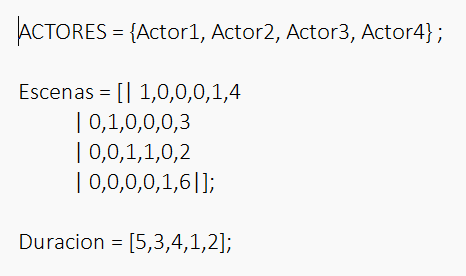
\includegraphics[width=0.35\textwidth]{img/test02_m1.png}
\end{center}

\subsubsection{test03_m1_a6_e6.dzn}
\begin{center}
    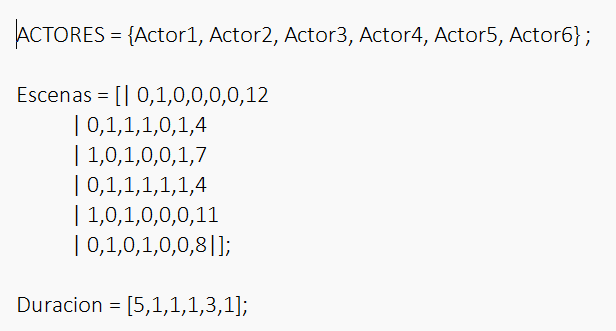
\includegraphics[width=0.35\textwidth]{img/test03_m1.png}
\end{center}

\subsubsection{test03_m1_a7_e9.dzn}
\begin{center}
    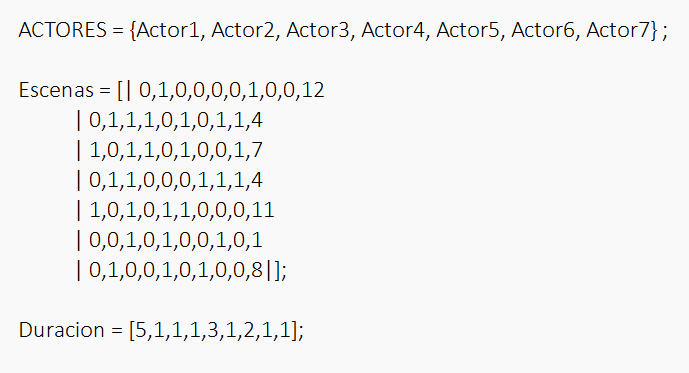
\includegraphics[width=0.35\textwidth]{img/test04_m1.png}
\end{center}

\subsection{Conclusiones}
\subsubsection{Pruebas de tiempo para el modelo básico}
\begin{center}
    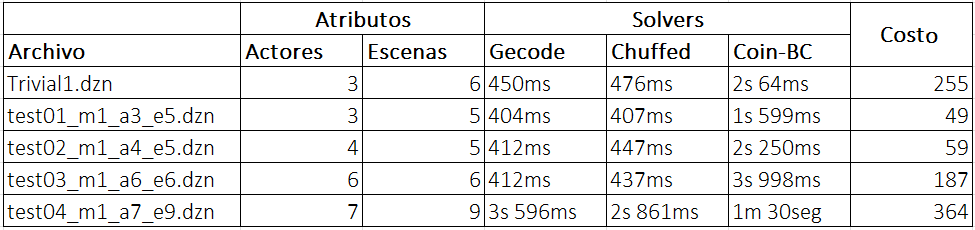
\includegraphics[width=0.8\textwidth]{img/pruebasModelo1.png}
\end{center}
Después de ejecutar las pruebas de los diferentes escenarios sobre el primer modelo del problema con tres diferentes solvers se puede evidenciar que $Gecode$ tiene un mejor tiempo promedio de solición seguido por $Chuffed$ y en el último puesto se tiene a $Coin-BC$. \newline\newline

Al tener un problema que se basa en el ordenamiento de las escenas llegamos a la conclusión que esta es la variable mas relevante que incide en el tiempo de solución del problema. Podríamos indicar a pesar que el número de actores de la prueba final es aproximadamente el doble de la cantidad de la prueba final, tener que ordenarlos en 1.5 veces mas el número de escenas tuvo un impacto notable en el rendimiento.

\subsection{Estrategias de distribución}
Analizando las estrategias de distribucióon se usó el solver Gecode Gist con su herramienta para visualizar la búsqueda que permite ver claramente las diferencias las distribuciones. Se uso el archivo de pruebas con mayor extenisión en actores y escenas.
\subsubsection{Nodos explorados para test04_m1_a7_e9.dzn}
\begin{center}
    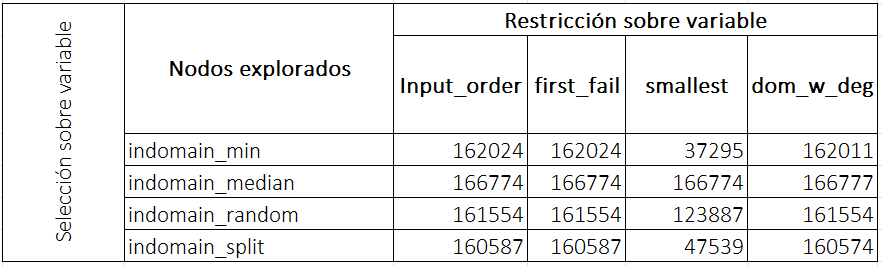
\includegraphics[width=0.80\textwidth]{img/estrategiasDeDistribucion.png}
\end{center}

\section{Modelo extendido}
A continuación se describe el contenido del modelo extendido. \newline

\subsection{Parámetros de entrada}
A las entradas del modelo básico se le adicionan los siguientes parámetros.
\begin{itemize}
    \item $Disponibilidad$: Es la información de las restricciones de los actores especificados en el conjunto de $ACTORES$. $Disponibilidad_{i,j}$ con $i \in [1..n\textunderscore actores]$ y con $j \in [1..2]$ representa la cantidad de horas máxima que actor $i$ de nombre $Disponibilidad_{i,1} \in ACTORES$ puede estár disponible para la grabación de la telenovela con tiempo $Disponibilidad_{i,2} \in \mathbb{N} $. El caso en que la disponibilidad del actor $i$  $Disponibilidad_{i,2} = 0$ significa que no tiene restricciones de tiempo.
    \item $Evitar:$ Es la información de las parejas de actores que no 
    pueden estar (cualquiera que sea la razón) en la misma escena donde $Evitar_{i,j}$ con $i \in \mathbb{N}$ y con $j \in [1..2]$ representa la información de una pareja con $Evitar_{i,1} \in ACTORES$ los primeros actores y $Evitar_{i,2} \in ACTORES$ los segundos actores.
\end{itemize}

\subsection{Variables}
A las variables del modelo básico se le agregan las siguientes:
\begin{itemize}
    \item $tiempo\textunderscore min\textunderscore x\textunderscore actor$: Son los tiempos mínimos que debe permanecer cada actor en las escenas para grabar donde $tiempo\textunderscore  x\textunderscore actor_i \in \mathbb{N}$ con $i \in [1..n\textunderscore actores]$ es el tiempo con respecto al orden inicial de las escenas, esta variable se usa para saber si las condiciones de $Disponibilidad$ pueden llegar a ser insactifactibles.
    \item $disponibilidad\textunderscore incumplida$: Es la información de los actores a los que la solución no les puede garantizar el cumplimiento de la restricción de disponibilidad donde $disponibilidad\textunderscore incumplida_i \in \{0,1\}$ con $i \in [1..n(Disponibilidad)]$ donde $1$ indica si la solución del problema incumple con la restricción de disponibilidad del actor $i$ y $0$ lo contrario.
    \item $evitar\textunderscore incumplida$: Es la información de los actores a los que la solución no les puede garantizar que se eviten; Por evitar se entiende que no asistan a la misma escena. $evitar\textunderscore incumplida_i \in \{0,1\}$ con $i \in [1..n(Evitar)]$ donde $1$ indica que no se puede garantizar que la pareja de actores $i$ se eviten y $0$ lo contrario.
\end{itemize}

\subsection{Restricciones}
A las restricciones del modelo básico se le agregan las siguientes:
\begin{itemize}
    \item $\forall i\sum_{j=1}^{n\textunderscore escenas}$  $Duracion_j * Escenas_{i,j} = tiempo\textunderscore min\textunderscore x\textunderscore actor$\newline
          donde $i \in [1..n\textunderscore actores]$.
    \item $\forall i$  if $Disponibilidad_{i,2} > 0$ then if $tiempo\textunderscore min\textunderscore x\textunderscore actor <= Disponibilidad_{i,2}$ then $tiempo\textunderscore min\textunderscore x\textunderscore actor <= Disponibilidad_{i,2}$ else $disponibilidad\textunderscore incumplida_i = 1$\newline
          donde $i \in [1..n(Disponibilidad)]$.
    \item $\forall j \forall i$ $evitar\textunderscore incumplida_j=1$   \newline donde $i \in [1..n\textunderscore escenas] \land j \in [1..n(Evitar)] \land Escenas[Evitar[j,1],i]=1 \land Escenas[Evitar[j,1],i]=Escenas[Evitar[j,2],i]$
\end{itemize}

\subsection{Función objetivo}
Al igual que la función objetivo del modelo básico, el modelo extendido intenta minimizar el costo total de la nómina de los actores a partir de la variable $costo\textunderscore x\textunderscore\ actor$
\begin{itemize}
    \item $min(\sum_{i=1}^{n\textunderscore actores}costo\textunderscore x\textunderscore actor$)
\end{itemize}

\subsection{Pruebas}
A continuación se presentan los escenarios de pruebas a los que se sometió el modelo usando Minizinc, el equipo usado para correr las pruebas tiene un procesador Intel(R) Core(TM) i7-10510U CPU @ 1.80GHz   2.30 GHz con 16.0 GB (15.8 GB usable) de RAM DDR4 bus 2400MHz.\newline
Se adjuntan los escenarios de prueba.

\subsubsection{test01_m2_a3_e5.dzn}
\begin{center}
    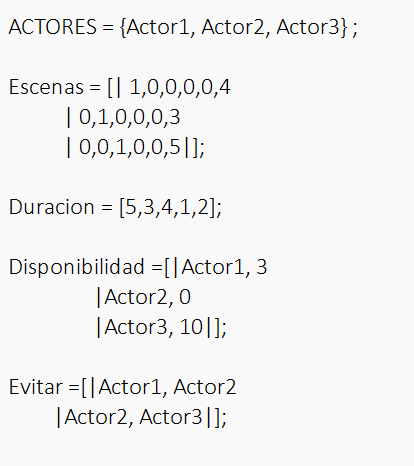
\includegraphics[width=0.35\textwidth]{img/test05_m2.png}
\end{center}

\subsubsection{test02_m2_a4_e5.dzn}
\begin{center}
    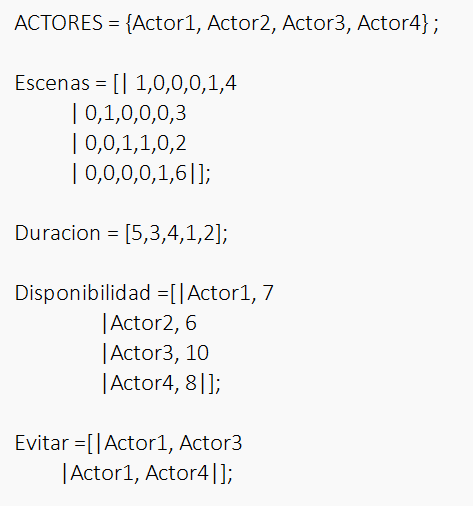
\includegraphics[width=0.35\textwidth]{img/test06_m2.png}
\end{center}

\subsubsection{test03_m2_a6_e6.dzn}
\begin{center}
    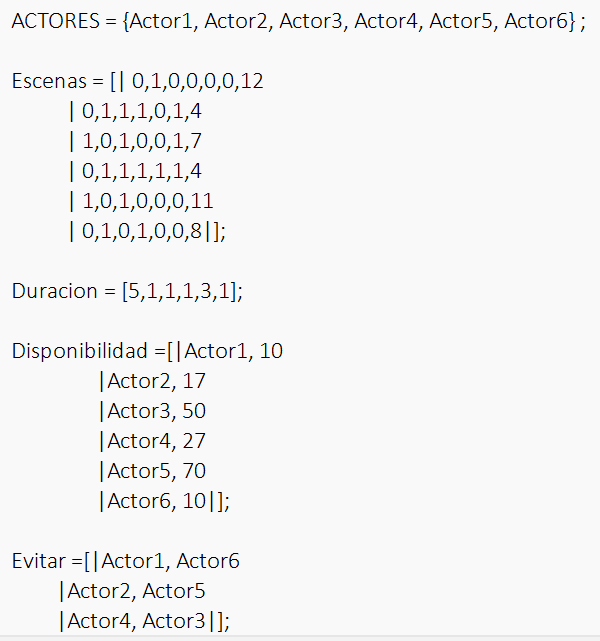
\includegraphics[width=0.35\textwidth]{img/test07_m2.png}
\end{center}

\subsubsection{test03_m2_a7_e9.dzn}
\begin{center}
    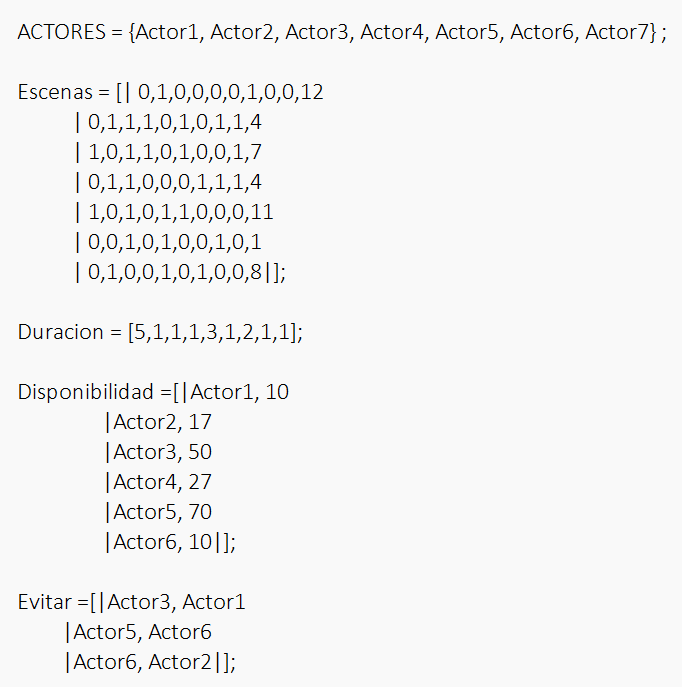
\includegraphics[width=0.35\textwidth]{img/test08_m2.png}
\end{center}

\subsection{Conclusiones}
\subsubsection{Pruebas de tiempo para el modelo extendido}
\begin{center}
    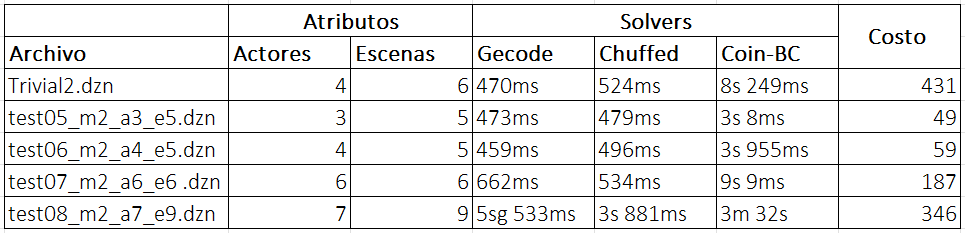
\includegraphics[width=0.8\textwidth]{img/pruebasModelo2.png}
\end{center}
Después de ejecutar las pruebas de los diferentes escenarios sobre el modelo extendido del problema con tres diferentes solvers se puede evidenciar que $Gecode$ tiene un mejor tiempo promedio de solición cuando el número de actores y escenas apenas se esta incrementando, luego $Chuffed$ toma la delantera en el mejor tiempo de solución. Por último y en todos los casos se tiene a $Coin-BC$. \newline\newline

Teniendo en cuenta que en algunos casos las restricciones adicionales generaron mas condiciones para hallar la mejor solución de cada problema podemos concluir que el tiempo de solución aumentó en aproximadamente el doble comparado con los escenarios del modelo inicial, el cual tenía la misma distribución de actores y escenas pero las dos restricciones adicionales de Disponibilidad y Evitar.

\section{Despliegue del proyeto}
El código fuente del proyecto se encuentra disponible en el repositorio de $GitHub$ \url{https://github.com/sebastianaf/ppr-project}, la versión funcional del código se encuentra desplegada en la web. Para accederla se debe tener en cuenta la siguiente información:\newline\newline

\subsection{Credenciales de acceso}
\textbf{Sitio web:} \url{https://ppr.enerfris.com}\newline
\textbf{Usuario:} admin\newline
\textbf{Contraseña:} ppr22
\newline\newline

El servidor con la aplicación web del proyecto está disponible de Lunes a Domingo de 8am a 12 am.

\end{document}